\documentclass[twoside]{book}

% Packages required by doxygen
\usepackage{fixltx2e}
\usepackage{calc}
\usepackage{doxygen}
\usepackage[export]{adjustbox} % also loads graphicx
\usepackage{graphicx}
\usepackage[utf8]{inputenc}
\usepackage{makeidx}
\usepackage{multicol}
\usepackage{multirow}
\PassOptionsToPackage{warn}{textcomp}
\usepackage{textcomp}
\usepackage[nointegrals]{wasysym}
\usepackage[table]{xcolor}

% Font selection
\usepackage[T1]{fontenc}
\usepackage[scaled=.90]{helvet}
\usepackage{courier}
\usepackage{amssymb}
\usepackage{sectsty}
\renewcommand{\familydefault}{\sfdefault}
\allsectionsfont{%
  \fontseries{bc}\selectfont%
  \color{darkgray}%
}
\renewcommand{\DoxyLabelFont}{%
  \fontseries{bc}\selectfont%
  \color{darkgray}%
}
\newcommand{\+}{\discretionary{\mbox{\scriptsize$\hookleftarrow$}}{}{}}

% Page & text layout
\usepackage{geometry}
\geometry{%
  a4paper,%
  top=2.5cm,%
  bottom=2.5cm,%
  left=2.5cm,%
  right=2.5cm%
}
\tolerance=750
\hfuzz=15pt
\hbadness=750
\setlength{\emergencystretch}{15pt}
\setlength{\parindent}{0cm}
\setlength{\parskip}{0.2cm}
\makeatletter
\renewcommand{\paragraph}{%
  \@startsection{paragraph}{4}{0ex}{-1.0ex}{1.0ex}{%
    \normalfont\normalsize\bfseries\SS@parafont%
  }%
}
\renewcommand{\subparagraph}{%
  \@startsection{subparagraph}{5}{0ex}{-1.0ex}{1.0ex}{%
    \normalfont\normalsize\bfseries\SS@subparafont%
  }%
}
\makeatother

% Headers & footers
\usepackage{fancyhdr}
\pagestyle{fancyplain}
\fancyhead[LE]{\fancyplain{}{\bfseries\thepage}}
\fancyhead[CE]{\fancyplain{}{}}
\fancyhead[RE]{\fancyplain{}{\bfseries\leftmark}}
\fancyhead[LO]{\fancyplain{}{\bfseries\rightmark}}
\fancyhead[CO]{\fancyplain{}{}}
\fancyhead[RO]{\fancyplain{}{\bfseries\thepage}}
\fancyfoot[LE]{\fancyplain{}{}}
\fancyfoot[CE]{\fancyplain{}{}}
\fancyfoot[RE]{\fancyplain{}{\bfseries\scriptsize Generated on Mon Nov 23 2015 23\+:49\+:30 for Techno\+Gym by Doxygen }}
\fancyfoot[LO]{\fancyplain{}{\bfseries\scriptsize Generated on Mon Nov 23 2015 23\+:49\+:30 for Techno\+Gym by Doxygen }}
\fancyfoot[CO]{\fancyplain{}{}}
\fancyfoot[RO]{\fancyplain{}{}}
\renewcommand{\footrulewidth}{0.4pt}
\renewcommand{\chaptermark}[1]{%
  \markboth{#1}{}%
}
\renewcommand{\sectionmark}[1]{%
  \markright{\thesection\ #1}%
}

% Indices & bibliography
\usepackage{natbib}
\usepackage[titles]{tocloft}
\setcounter{tocdepth}{3}
\setcounter{secnumdepth}{5}
\makeindex

% Hyperlinks (required, but should be loaded last)
\usepackage{ifpdf}
\ifpdf
  \usepackage[pdftex,pagebackref=true]{hyperref}
\else
  \usepackage[ps2pdf,pagebackref=true]{hyperref}
\fi
\hypersetup{%
  colorlinks=true,%
  linkcolor=blue,%
  citecolor=blue,%
  unicode%
}

% Custom commands
\newcommand{\clearemptydoublepage}{%
  \newpage{\pagestyle{empty}\cleardoublepage}%
}


%===== C O N T E N T S =====

\begin{document}

% Titlepage & ToC
\hypersetup{pageanchor=false,
             bookmarks=true,
             bookmarksnumbered=true,
             pdfencoding=unicode
            }
\pagenumbering{roman}
\begin{titlepage}
\vspace*{7cm}
\begin{center}%
{\Large Techno\+Gym }\\
\vspace*{1cm}
{\large Generated by Doxygen 1.8.10}\\
\vspace*{0.5cm}
{\small Mon Nov 23 2015 23:49:30}\\
\end{center}
\end{titlepage}
\clearemptydoublepage
\tableofcontents
\clearemptydoublepage
\pagenumbering{arabic}
\hypersetup{pageanchor=true}

%--- Begin generated contents ---
\chapter{S\+E\+N\+G330\+\_\+\+Ass2}
\label{md__r_e_a_d_m_e}
\hypertarget{md__r_e_a_d_m_e}{}
Assignment 2 for S\+E\+N\+G330 Fall 2015 
\chapter{Hierarchical Index}
\section{Class Hierarchy}
This inheritance list is sorted roughly, but not completely, alphabetically\+:\begin{DoxyCompactList}
\item Cloneable\begin{DoxyCompactList}
\item \contentsline{section}{Equipment}{\pageref{interface_equipment}}{}
\begin{DoxyCompactList}
\item \contentsline{section}{Elliptical}{\pageref{class_elliptical}}{}
\item \contentsline{section}{Treadmill}{\pageref{class_treadmill}}{}
\end{DoxyCompactList}
\end{DoxyCompactList}
\item \contentsline{section}{Clone\+Factory}{\pageref{class_clone_factory}}{}
\item \contentsline{section}{Techno\+Gym}{\pageref{class_techno_gym}}{}
\end{DoxyCompactList}

\chapter{Class Index}
\section{Class List}
Here are the classes, structs, unions and interfaces with brief descriptions\+:\begin{DoxyCompactList}
\item\contentsline{section}{\hyperlink{class_clone_factory}{Clone\+Factory} }{\pageref{class_clone_factory}}{}
\item\contentsline{section}{\hyperlink{class_elliptical}{Elliptical} }{\pageref{class_elliptical}}{}
\item\contentsline{section}{\hyperlink{interface_equipment}{Equipment} }{\pageref{interface_equipment}}{}
\item\contentsline{section}{\hyperlink{class_techno_gym}{Techno\+Gym} }{\pageref{class_techno_gym}}{}
\item\contentsline{section}{\hyperlink{class_treadmill}{Treadmill} }{\pageref{class_treadmill}}{}
\end{DoxyCompactList}

\chapter{Class Documentation}
\hypertarget{class_clone_factory}{}\section{Clone\+Factory Class Reference}
\label{class_clone_factory}\index{Clone\+Factory@{Clone\+Factory}}
\subsection*{Public Member Functions}
\begin{DoxyCompactItemize}
\item 
\hyperlink{interface_equipment}{Equipment} \hyperlink{class_clone_factory_a2d6a40c6aab4cde2cf14c34accf11dcf}{get\+Clone} (\hyperlink{interface_equipment}{Equipment} equipment)
\end{DoxyCompactItemize}


\subsection{Detailed Description}
A class that clones equipment regaurdless of the subtype \begin{DoxyAuthor}{Author}
Greg bacic 
\end{DoxyAuthor}


\subsection{Member Function Documentation}
\hypertarget{class_clone_factory_a2d6a40c6aab4cde2cf14c34accf11dcf}{}\index{Clone\+Factory@{Clone\+Factory}!get\+Clone@{get\+Clone}}
\index{get\+Clone@{get\+Clone}!Clone\+Factory@{Clone\+Factory}}
\subsubsection[{get\+Clone(\+Equipment equipment)}]{\setlength{\rightskip}{0pt plus 5cm}{\bf Equipment} Clone\+Factory.\+get\+Clone (
\begin{DoxyParamCaption}
\item[{{\bf Equipment}}]{equipment}
\end{DoxyParamCaption}
)\hspace{0.3cm}{\ttfamily [inline]}}\label{class_clone_factory_a2d6a40c6aab4cde2cf14c34accf11dcf}
Makes a clone of the original equipment reguardless of subclass 
\begin{DoxyParams}{Parameters}
{\em equipment} & with tipe \hyperlink{class_elliptical}{Elliptical} or \hyperlink{class_treadmill}{Treadmill} \\
\hline
\end{DoxyParams}
\begin{DoxyReturn}{Returns}
copy of equipment w will be located at different memoery adddress, not a pass by reference but as copy 
\end{DoxyReturn}


The documentation for this class was generated from the following file\+:\begin{DoxyCompactItemize}
\item 
Clone\+Factory.\+java\end{DoxyCompactItemize}

\hypertarget{class_elliptical}{}\section{Elliptical Class Reference}
\label{class_elliptical}\index{Elliptical@{Elliptical}}
Inheritance diagram for Elliptical\+:\begin{figure}[H]
\begin{center}
\leavevmode
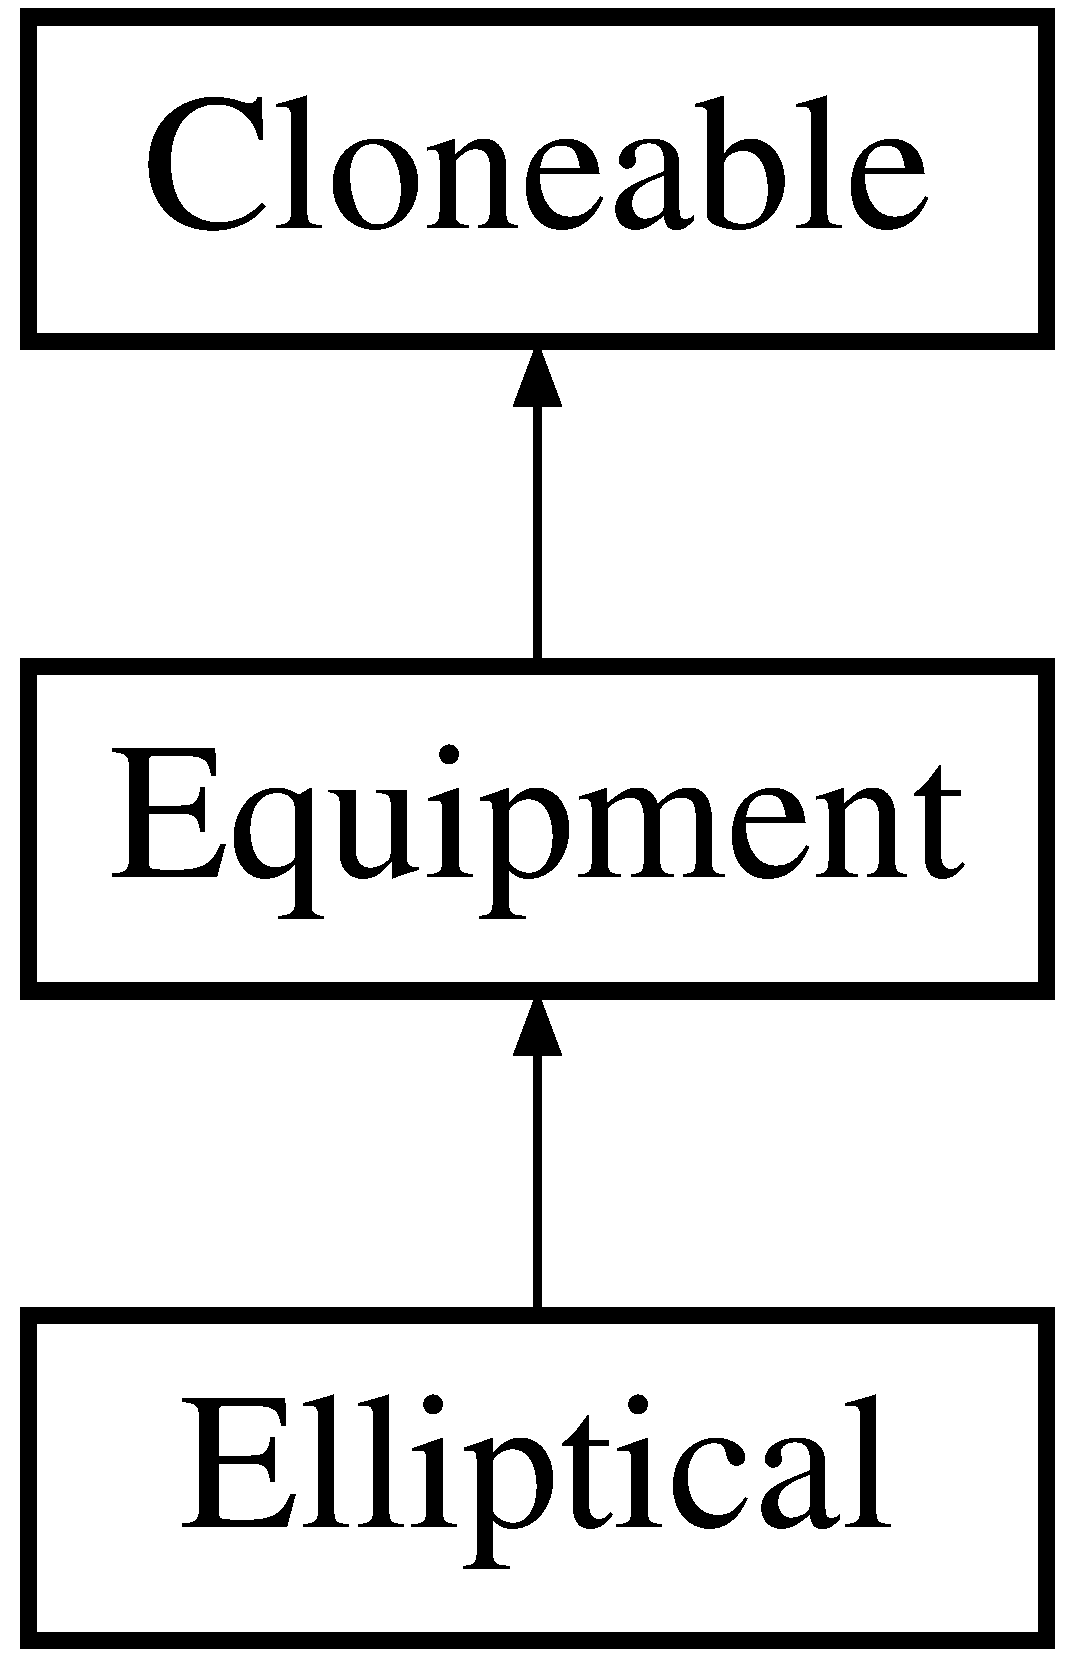
\includegraphics[height=3.000000cm]{class_elliptical}
\end{center}
\end{figure}
\subsection*{Public Member Functions}
\begin{DoxyCompactItemize}
\item 
\hyperlink{class_elliptical_a104d7a8d5a0ae148b626ed7c7ce5f800}{Elliptical} (int id, String location)
\item 
\hyperlink{class_elliptical}{Elliptical} \hyperlink{class_elliptical_a3d177b724814a280c13c826b027abb86}{make\+Copy} ()
\item 
String \hyperlink{class_elliptical_a4e61075ac315a42ab13b1d4bc70ae066}{to\+String} ()
\end{DoxyCompactItemize}


\subsection{Constructor \& Destructor Documentation}
\hypertarget{class_elliptical_a104d7a8d5a0ae148b626ed7c7ce5f800}{}\index{Elliptical@{Elliptical}!Elliptical@{Elliptical}}
\index{Elliptical@{Elliptical}!Elliptical@{Elliptical}}
\subsubsection[{Elliptical(int id, String location)}]{\setlength{\rightskip}{0pt plus 5cm}Elliptical.\+Elliptical (
\begin{DoxyParamCaption}
\item[{int}]{id, }
\item[{String}]{location}
\end{DoxyParamCaption}
)\hspace{0.3cm}{\ttfamily [inline]}}\label{class_elliptical_a104d7a8d5a0ae148b626ed7c7ce5f800}
Constructor for \hyperlink{class_elliptical}{Elliptical} which inherits properties from equipment 
\begin{DoxyParams}{Parameters}
{\em id} & an integer that will be used as the equipment I\+D \\
\hline
{\em location} & a string for the location of the eqipment \\
\hline
\end{DoxyParams}


\subsection{Member Function Documentation}
\hypertarget{class_elliptical_a3d177b724814a280c13c826b027abb86}{}\index{Elliptical@{Elliptical}!make\+Copy@{make\+Copy}}
\index{make\+Copy@{make\+Copy}!Elliptical@{Elliptical}}
\subsubsection[{make\+Copy()}]{\setlength{\rightskip}{0pt plus 5cm}{\bf Elliptical} Elliptical.\+make\+Copy (
\begin{DoxyParamCaption}
{}
\end{DoxyParamCaption}
)\hspace{0.3cm}{\ttfamily [inline]}}\label{class_elliptical_a3d177b724814a280c13c826b027abb86}
\hyperlink{class_elliptical}{Elliptical} copy make a clone of the elliptical obkect and is called from Clonefactory 
\begin{DoxyExceptions}{Exceptions}
{\em Clone\+Not\+Supported} & excepion thrown if \hyperlink{interface_equipment}{Equipment} does not extend Cloneable \\
\hline
\end{DoxyExceptions}


Implements \hyperlink{interface_equipment}{Equipment}.

\hypertarget{class_elliptical_a4e61075ac315a42ab13b1d4bc70ae066}{}\index{Elliptical@{Elliptical}!to\+String@{to\+String}}
\index{to\+String@{to\+String}!Elliptical@{Elliptical}}
\subsubsection[{to\+String()}]{\setlength{\rightskip}{0pt plus 5cm}String Elliptical.\+to\+String (
\begin{DoxyParamCaption}
{}
\end{DoxyParamCaption}
)\hspace{0.3cm}{\ttfamily [inline]}}\label{class_elliptical_a4e61075ac315a42ab13b1d4bc70ae066}
Default java to\+String method. outputs information to console; 

The documentation for this class was generated from the following file\+:\begin{DoxyCompactItemize}
\item 
Elliptical.\+java\end{DoxyCompactItemize}

\hypertarget{interface_equipment}{}\section{Equipment Interface Reference}
\label{interface_equipment}\index{Equipment@{Equipment}}
Inheritance diagram for Equipment\+:\begin{figure}[H]
\begin{center}
\leavevmode
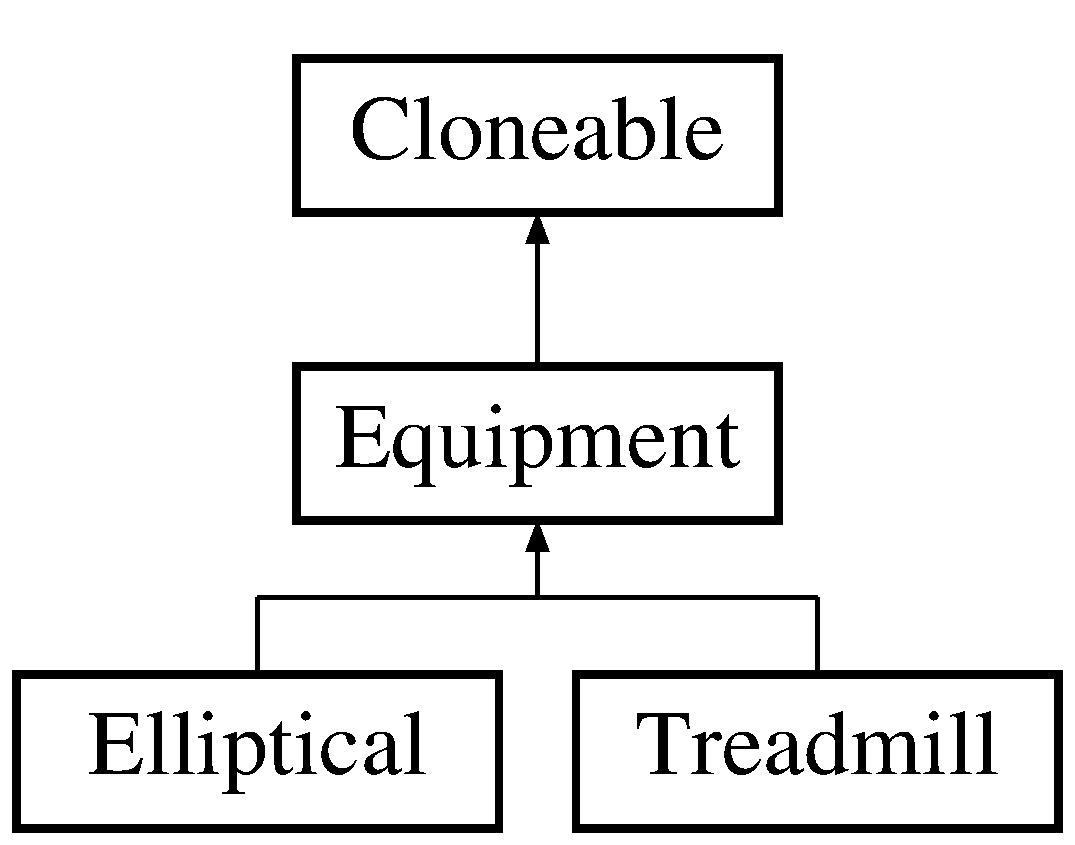
\includegraphics[height=3.000000cm]{interface_equipment}
\end{center}
\end{figure}
\subsection*{Public Member Functions}
\begin{DoxyCompactItemize}
\item 
\hypertarget{interface_equipment_aec219eb46c6185f11c174c95a582f2eb}{}\hyperlink{interface_equipment}{Equipment} {\bfseries make\+Copy} ()\label{interface_equipment_aec219eb46c6185f11c174c95a582f2eb}

\end{DoxyCompactItemize}


\subsection{Detailed Description}
A class that extends the java cloneable object and makes a copy of an existing objects, regardless of subtype. \begin{DoxyAuthor}{Author}
Greg bacic 
\end{DoxyAuthor}


The documentation for this interface was generated from the following file\+:\begin{DoxyCompactItemize}
\item 
Equipment.\+java\end{DoxyCompactItemize}

\hypertarget{class_techno_gym}{}\section{Techno\+Gym Class Reference}
\label{class_techno_gym}\index{Techno\+Gym@{Techno\+Gym}}
\subsection*{Static Public Member Functions}
\begin{DoxyCompactItemize}
\item 
\hypertarget{class_techno_gym_a69e68d6c95e9fa3806b94b6de51908c3}{}static void {\bfseries main} (String\mbox{[}$\,$\mbox{]} Args)\label{class_techno_gym_a69e68d6c95e9fa3806b94b6de51908c3}

\end{DoxyCompactItemize}


The documentation for this class was generated from the following file\+:\begin{DoxyCompactItemize}
\item 
Techno\+Gym.\+java\end{DoxyCompactItemize}

\hypertarget{class_treadmill}{}\section{Treadmill Class Reference}
\label{class_treadmill}\index{Treadmill@{Treadmill}}
Inheritance diagram for Treadmill\+:\begin{figure}[H]
\begin{center}
\leavevmode
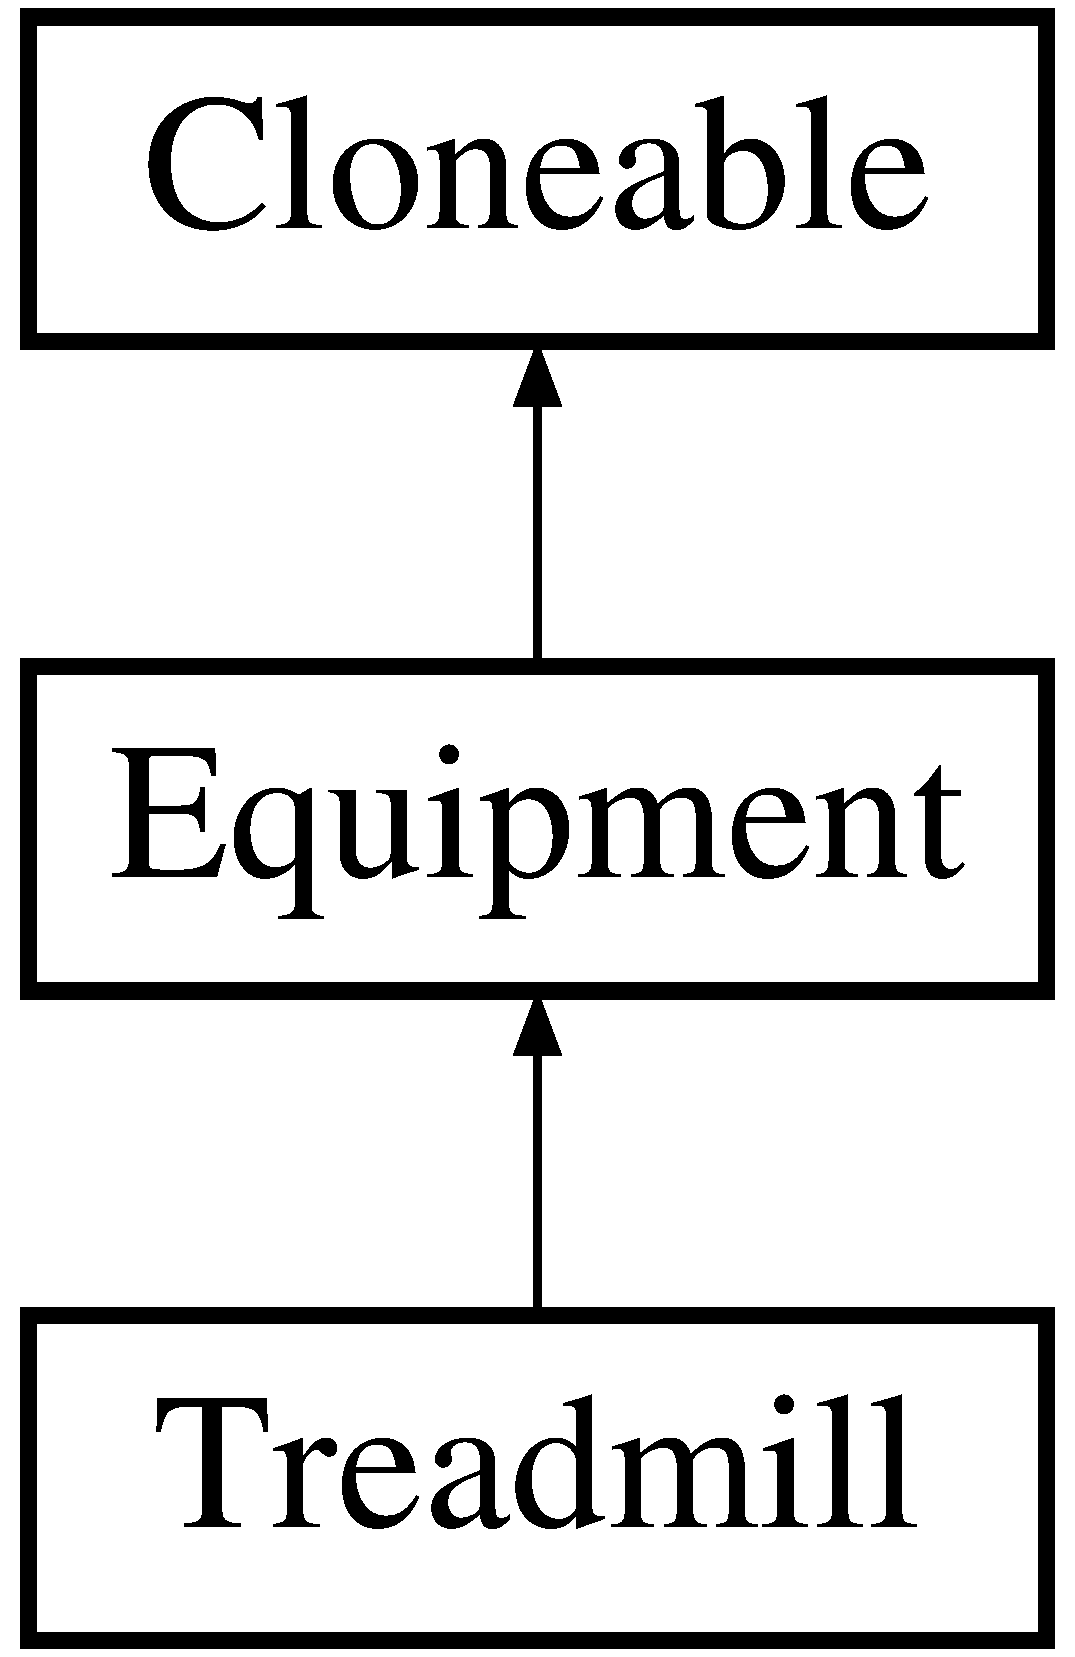
\includegraphics[height=3.000000cm]{class_treadmill}
\end{center}
\end{figure}
\subsection*{Public Member Functions}
\begin{DoxyCompactItemize}
\item 
\hyperlink{class_treadmill_a73abf72303a3448bb81f572e4d29d595}{Treadmill} (int id, String location)
\item 
\hyperlink{class_treadmill}{Treadmill} \hyperlink{class_treadmill_a3431c4cc70cd2b6e9414df628eff7997}{make\+Copy} ()
\item 
String \hyperlink{class_treadmill_a73b6c456c73c8188db6c5d4deef1522e}{to\+String} ()
\end{DoxyCompactItemize}


\subsection{Detailed Description}
The \hyperlink{class_treadmill}{Treadmill} class which inherits make\+Copy from \hyperlink{interface_equipment}{Equipment} \begin{DoxyAuthor}{Author}
Greg bacic 
\end{DoxyAuthor}


\subsection{Constructor \& Destructor Documentation}
\hypertarget{class_treadmill_a73abf72303a3448bb81f572e4d29d595}{}\index{Treadmill@{Treadmill}!Treadmill@{Treadmill}}
\index{Treadmill@{Treadmill}!Treadmill@{Treadmill}}
\subsubsection[{Treadmill(int id, String location)}]{\setlength{\rightskip}{0pt plus 5cm}Treadmill.\+Treadmill (
\begin{DoxyParamCaption}
\item[{int}]{id, }
\item[{String}]{location}
\end{DoxyParamCaption}
)\hspace{0.3cm}{\ttfamily [inline]}}\label{class_treadmill_a73abf72303a3448bb81f572e4d29d595}
Constructor for \hyperlink{class_treadmill}{Treadmill} which inherits properties from equipment 
\begin{DoxyParams}{Parameters}
{\em id} & an integer that will be used as the equipment I\+D \\
\hline
{\em location} & a string for the location of the eqipment \\
\hline
\end{DoxyParams}


\subsection{Member Function Documentation}
\hypertarget{class_treadmill_a3431c4cc70cd2b6e9414df628eff7997}{}\index{Treadmill@{Treadmill}!make\+Copy@{make\+Copy}}
\index{make\+Copy@{make\+Copy}!Treadmill@{Treadmill}}
\subsubsection[{make\+Copy()}]{\setlength{\rightskip}{0pt plus 5cm}{\bf Treadmill} Treadmill.\+make\+Copy (
\begin{DoxyParamCaption}
{}
\end{DoxyParamCaption}
)\hspace{0.3cm}{\ttfamily [inline]}}\label{class_treadmill_a3431c4cc70cd2b6e9414df628eff7997}
\hyperlink{class_treadmill}{Treadmill} copy make a clone of the elliptical obkect and is called from Clonefactory 
\begin{DoxyExceptions}{Exceptions}
{\em Clone\+Not\+Supported} & excepion thrown if \hyperlink{interface_equipment}{Equipment} does not extend Cloneable \\
\hline
\end{DoxyExceptions}


Implements \hyperlink{interface_equipment}{Equipment}.

\hypertarget{class_treadmill_a73b6c456c73c8188db6c5d4deef1522e}{}\index{Treadmill@{Treadmill}!to\+String@{to\+String}}
\index{to\+String@{to\+String}!Treadmill@{Treadmill}}
\subsubsection[{to\+String()}]{\setlength{\rightskip}{0pt plus 5cm}String Treadmill.\+to\+String (
\begin{DoxyParamCaption}
{}
\end{DoxyParamCaption}
)\hspace{0.3cm}{\ttfamily [inline]}}\label{class_treadmill_a73b6c456c73c8188db6c5d4deef1522e}
Default java to\+String method. outputs information to console; 

The documentation for this class was generated from the following file\+:\begin{DoxyCompactItemize}
\item 
Treadmill.\+java\end{DoxyCompactItemize}

%--- End generated contents ---

% Index
\backmatter
\newpage
\phantomsection
\clearemptydoublepage
\addcontentsline{toc}{chapter}{Index}
\printindex

\end{document}
